\chapter{Постановка задачи и обзор литературы} \label{ch1}
\section{Постановка задачи} \label{ch1:sec1}
\par Исходные изображения, наблюдаемые с микроскопа, крайне неточны - содержат шумы и искажения из-за несовершенства системы регистрации и волновой природы света. Получаемое изображение $I_y$ является результатом свёртки (конволюции) точного объекта $I_x$ с функцией рассеяния точки (ФРТ) системы $H$ , которая его формирует. [*] Помимо этого, важно помнить, что системы регистрации изображения, в рамках данной задачи конфокальной микроскопии, вносят добавочный фотонный шум $N$. Схема получения наблюдаемого изображения приведено на \firef{fig:problem-start}. Формальная запись наблюдаемого изображения будет выглядеть следующим образом:
\begin{equation}\label{eq:problem}
	I_y = I_x \circledast H + N
\end{equation}
где $I_x$ - точное изображение объекта, $I_x \in \Omega_x$ - множество точных изображений объектов, $I_y$ - наблюдаемое изображение объекта $I_y \in \Omega_y$ - множество наблюдаемых изображений объектов, $H$ - функция рассеивания точки, $N$ - шум, вносимый регистрируемым прибором, $\circledast$ - операция свёртки.
\begin{minipage}{\textwidth}
	\centering
	\vspace{\mfloatsep} % интервал  	
	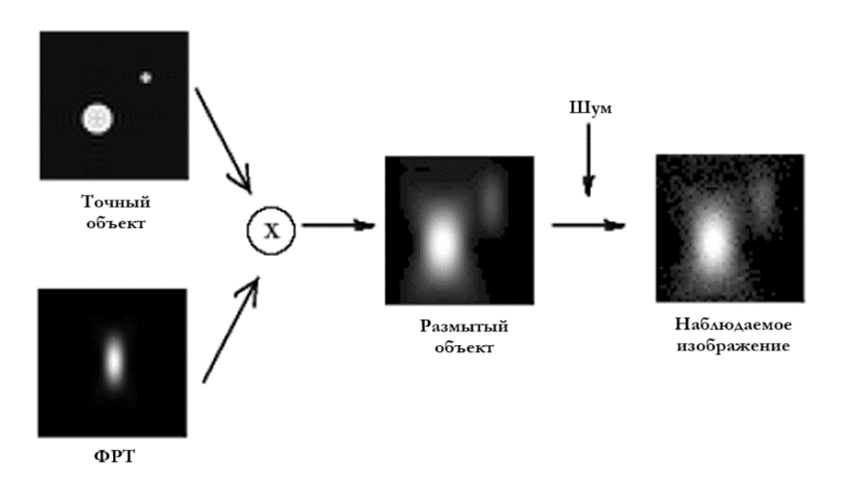
\includegraphics[keepaspectratio=true,scale=0.55] {my_folder/images/problem/start.png}
	\captionof{figure}{Схема свёртки точного объекта с ФРТ вместе с фотонным шумом}\label{fig:problem-start}  
	\vspace{\mfloatsep} % интервал  	
\end{minipage}
\par Не умоляя общности, рассмотрим изображения $I_x, I_y$, как дискретный набор значений. Тогда множества $\Omega_x, \Omega_y$ могут быть представлены, как пространства $\mathbb{R}^{l,r,c}$, где $l, r, c$ - число слоёв, высота и ширина каждого слоя изображения. В случае наличия нескольких каналов (например, $w$), пространства могуть быть представлены, как $\mathbb{R}^{l,r,c,w}$. Также важно отметить, что шум $N$ рассматривается, как элемент пространства $\mathbb{R}^{l,r,c} (\mathbb{R}^{l,r,c,w})$. Подробнее о природе шума и постановке задачи денойзинга будет рассмотрено в следующем пункте.
\par Методы восстановления "точного" изображения по наблюдаемому называются \textit{деконволюцией} (процесс обратный к свёртке). Общая задача восстановления изображения может быть сведена к выбору функции $\mathscr{F}(I_y)$:
\begin{equation}
	\hat{I_x} = \mathscr{F}(I_y)
\end{equation}
где $\hat{I_x}$ - аппрокимация $I_x, \hat{I_x} \in \Omega_x$
\par Однако зачастую процесс восстановления изображений рассматривается как два последовательных этапа: денойзинг (обесшумливание) изображений и сама деконволюция (т.е. процесс улучшения качества размытого снимка некоторого образца). Это обусловлено тем, что методы деконволюции искажают снимки при наличии шума.

\subsection{Постановка задачи денойзинга}
\par Флуоресцентная микроскопия характеризуется пуассоновско-гауссовым шумом (mixed Poisson–Gaussian, MPG), где пуассоновский шум является доминирующим источником шума.[2] Это объясняется тем, что количество фотонов, захваченных микроскопом, черезвычайно мало. Следовательно, измеренный оптический сигнал во флуоресцентной микроскопии квантуется из-за дискретной природы фотонов, и в изображениях, полученных с помощью флуоресцентной микроскопии, преобладает пуассоновский шум, а не гауссовский шум, который характерен для фотографии[*]. 
\par Шум может существенно ухудшать качество изображений и затруднять дальнейший анализ. Поэтому важно разработать алгоритм денойзинга, который будет эффективно удалять шум, сохраняя при этом важные структурные детали образцов.
\par Введём формальные обозначения для постановки задачи. Пусть $I_z = I_x * H$ - размытое изображение (свёртка точного объекта и ФРТ), не содержащая шумов. $I_z \in \Omega_z, \Omega_z \in \mathbb{R}^{l,r,c} (\mathbb{R}^{l,r,c,w})$ - множество размытых изображений объектов. Тогда задача денойзинга сводится к нахождению такой функции $\mathscr{F}_1(I_y)$, что:
\begin{equation}
	\hat{I_z} = \mathscr{F}_1(I_y)
\end{equation}
где $\hat{I_z}$ - аппрокимация $I_z, \hat{I_x} \in \Omega_x$.\\
Задача деконволюции сводится к поиску функции $\mathscr{F}_2(I_z)$: 
\begin{equation}
	\hat{I_x} = \mathscr{F}_2(I_z)
\end{equation}
где $\hat{I_x}$ - аппрокимация $I_x, \hat{I_x} \in \Omega_x$.\\
Общая задача восстановления изображений выглядит следующим образом:
\begin{equation}
	\hat{I_x} = \mathscr{F}_2(\mathscr{F}_1(I_y))
\end{equation}

Задача денойзинга трёхмерных изображений формулируется следующим образом:
\begin{itemize}[]
	\item Разработать алгоритм денойзинга трёхмерных изображений, где на вход поступает шумное изображение $I_y \in \mathbb{R}^{l,r,c}$, а на выходе получаем результат денойзинга: $I_z \in \mathbb{R}^{l,r,c}$ (см. \firef{fig:denoise-problem}).
	\item Исследовать природу шума на реальных снимках с конфокальных микроскопов и доказать эксперементальным способом, что он распределяется в большей мере по Пуассону с некоторым параметром $\lambda$:
	\begin{equation}
		P(\lambda) = \frac{\lambda^k e^{-\lambda}}{k!}
	\end{equation}
	где $\lambda$ - частота возникновения, уровень шума, $k$ - наблюдаемое значение случайной величины.
	
\end{itemize}
\begin{minipage}{\textwidth}
	\centering
	\vspace{\mfloatsep} % интервал  	
	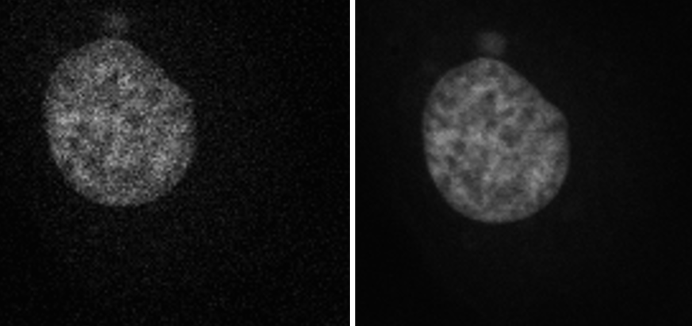
\includegraphics[keepaspectratio=true,scale=0.45] {my_folder/images/problem/denoisiong_example.png}
	\captionof{figure}{Пример работы денойзинга: слева - шумное изображение клетки, справа - обесшумленное (результат денойзинга)}\label{fig:denoise-problem} 
	\vspace{\mfloatsep} % интервал  	
\end{minipage}

\subsection{Постановка задачи автоматической сегментации сфер}
\par Для восстановления исходного изображения с помощью итерационных методов деконволюции необходимо в явном виде нахождение ФРТ. На практике точное значение ядра свёртки $H$ найти очень сложно, поэтому используют приближенное значение. Методы, создающие такие приближения, делятся на две группы: теоретические и экспериментальные.

\par Теоретические методы вычисляют ФРТ на основе определенных моделей и функций, тогда как экспериментальные методы включают съемку объектов очень малого размера, например, калибровочных флуоресцентных сфер. Функции рассеяния точки, полученные теоретическим путем, называют теоретическими ФРТ (тФРТ), а функции, полученные экспериментальным путем, — экспериментальными ФРТ (эФРТ). Оба метода обладают своими преимуществами и недостатками: так, например, теоретическая ФРТ не содержит шумов, которые могли бы приводить к неточностям при деконволюции, однако она же не отражает неточностей системы регистрации. Эксперементальный способ вычисления ФРТ имеет абсолютно обратные свойства.

\par Построение эФРТ происходит путём деконволюции размытой сферы, полученной из усреднения множества исходных, наблюдаемых с микроскопа снимков сфер, точным моделируемым изображением сферы. Более наглядное описание см на \firef{fig:autosegm-problem}. Стоит отметить тот факт, что чем больше размытых микроскопом снимков сфер участвует в усреднении, тем точнее получается эФРТ и, как следствие, результаты  аналитической деконволюции. Однако при извлечении большого количества сфер (80-100 и более), процесс сегментации может занять около 10-15 минут. Поэтому необходим автоматический подход, использующий методы компьютерного зрения, который позволил бы ускорить данный процесс, а также оставил возможность ручной корректировки результатов.
\begin{minipage}{\textwidth}
	\centering
	\vspace{\mfloatsep} % интервал  	
	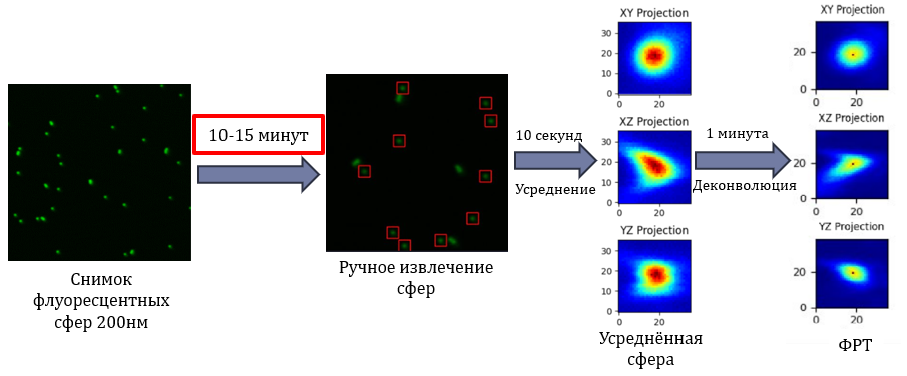
\includegraphics[keepaspectratio=true,scale=0.85] {my_folder/images/problem/segment_spheres.png}
	\captionof{figure}{Схема эксперементального способа вычисления ФРТ}\label{fig:autosegm-problem}  
	\vspace{\mfloatsep} % интервал  	
\end{minipage}

\section{Обзор литературы} \label{ch1:sec2}
\par В данном параграфе рассмотрено 2 ключевых подхода, которые будут использоваться для описания существующих методов, так и создания новых в следующей главе.
\subsection{Существующие методы деконволюции} 
\par \textit{Деконволюция} - это процесс восстановления оригинального изображения, которое было искажено в процессе съёмки. Глобально эти методы можно разбить на 2 группы: использующие функцию рассеяния точки ($H$) в процессе обработки, и не использующие. Вторую группу называют \textit{методами "слепой" деконволюции}, обычно дают менее точные результаты, если сравнивать с первой группой.
\par Рассмотрим подкласс алгоритмов первой группы, основанных на природе шума, которые называются \textit{статистические алгоритмы деконволюции}. Данный подкласс получен из алгоритма оценки максимального правдоподобия (MLE), написанного для минимизации пуассоновского шума на изображении[*]. 

\par \textit{Метод Ричардсона-Люси (RL)} основан на методе максимального правдоподобия и предназначен для работы с шумами, следующими закону распределения Пуассона. Этот алгоритм итеративно улучшает оценку объекта, исходя из текущей оценки, наблюдаемого изображения и известной ФРТ.
\begin{equation}
	\hat I^{k+1}_x = I^{k}_x(\frac{I_z}{I^{k}_x\circledast H})\circledast H^*
\end{equation}
где $I^k_x$ - текущее приближение на итерации k, $I_z$ - наблюдаемое (размытое) изображение, $H$ – функция рассеяния точки, $H^*$ - обратное ядро свёртки (ФРТ, повёрнутая относительно начала координат на 180 градусов).
\par Этот алгоритм обладает свойством неотрицательности, т.е. если начальное значение неотрицательно, то и все последующие итерации будут неотрицательными. Однако, при наличии шума алгоритм может сходиться к решению, доминируемому шумом, что ухудшает качество изображения. Помимо использования методов денойзинга для решения проблемы усиления шума, существуют модификации RL-алгоритма с добавлением регуляризационных членов. Разберём наиболее часто используемые модификации:
\begin{enumerate}[]
	\item \textit{Регуляризация Тихонова-Миллера (TM)}:\\
	\begin{equation}
		\hat I^{k+1}_x = I^{k}_x(\frac{I_z}{I^{k}_x\circledast H}\circledast H^*)\cdot(1 - 2\lambda_{TM}\nabla^2 I^{k}_x)
	\end{equation}
	где $\lambda_{TV}$ - параметр регуляризации, а $\nabla^2$ - лапласиан объекта.
	\item Общая вариация(Total variation, TV):\\
	TV-регуляризация сохраняет контуры и границы объектов, уменьшая шум в однородных областях.
	\begin{equation}
		TV(I_x) = \int |\nabla I_x| \, dxdydz
	\end{equation}
	\begin{equation}
		\hat I^{k+1}_x = I^{k}_x(\frac{I_z}{I^{k}_x\circledast H}\circledast H^*) - \lambda_{TV}\cdot TV(I^{k}_x)
	\end{equation}
	где $\lambda_{TV}$ - параметр регуляризации.
\end{enumerate}

\subsection{Элементы свёрточных нейронных сетей}
\par В данном подпараграфе будет представлен краткий обзор архитектурных элементов свёрточных нейронных сетей (CNN), которые играют ключевую роль в обработке и анализе изображений. 

\subsubsection{Свёрточный слой}
\par \textit{Свёрточный слой (Convolutional Layer)} является ключевым элементом CNN, часто используется для обработки изображений. Этот слой выполняет операцию свёртки (convolution), которая позволяет извлекать различные признаки из входных данных.
\par Операция свёртки двух функций $f$ и $g$ записывается так:
\begin{equation}
	(f*g)(x) = \int_{\mathbb{R^n}}^{} f(y)g(x-y)\,dy
\end{equation}
где $f,g: \mathbb{R^n} \Rightarrow \mathbb{R}$ - интегрируемые функции по мере Лебега на $\mathbb{R}^n$, а $(f*g)(x): \mathbb{R^n} \Rightarrow \mathbb{R}$.
Назовём $f(x)$ вход, $g(x)$ - ядро, а результат $(f*g)(x)$ - карта признаков.
\par Распишем понятния в рамках нашей задчи:\\
\textit{Фильтр(ядро свёртки)} – это матрица небольшого размера, которая скользит по изображению и выполняет операцию свёртки. Пусть задана размером $k \times k$.
\textit{Свёртка} - это операция, при которой фильтр скользит по входному изображению и вычисляет сумму произведений элементов фильтра и соответствующих элементов области изображения. Если входное изображение имеет размер $r \times c$ и фильтр $k \times k$, то выходное будет иметь размер $(r-k+1) \times (c-k+1)$ без применения дополнения (\textit{padding}). Если у нас n фильтров, то рамзер будет: $(r-k+1) \times (c-k+1) \times n$.
\par Свёрточные слои могут иметь несколько каналов. В этом случае, каждый канал имеет свой собственный фильтр, и результаты свёртки с каждым каналом суммируются.
\par Рассмотрим формулу свёрточного слоя двухмерного изображения с одним фильтром и одним каналом изображения.
\begin{equation}
	O(i,j) = (I*K)(i,j) = \sum_{u=0}^{k-1}\sum_{v=0}^{k-1}I(i+u, j+v) \cdot K(u,v)
\end{equation}
где $I$ - входное изображение размером $r \times c$, $K$ -фильтр размером $k \times k$, $O$ - выходное изображение, результат свёртки, $i=0,1,.., r-k$ и $j=0,1,.., c-k$ - точки карты признаков.
\par Также рассмотрим применения "дополнения" (Padding) и "шага" (Stride) для свёрточных слоёв:
\begin{enumerate}[]
	\item Padding добавляет рамку из нулей вокруг входного изображения, чтобы контролировать размер выходного изображения. Например, чтобы сохранить размер выходного изображения, если применить $p = \frac{k-1}{2}$, для фильтра размером $k \times k$
	\item Stride – это шаг, с которым фильтр скользит по изображению. Если шаг равен 
	$s$, то выходное изображение будет иметь размер:
	\begin{equation}
		(\frac{r-k}{s}) + 1 \times (\frac{c-k}{s}) + 1 
	\end{equation}
\end{enumerate}

\subsubsection{Слой объединения (Pooling-слой)}
\par \textit{Слой объединения (Pooling Layer)} используется для уменьшения пространственных размеров карт признаков и количества параметров, сохраняя при этом наиболее важную информацию. 
\par Наиболее распространённые слои объединения:
\begin{itemize}[]
	\item Максимальное объединение (Max Pooling). Этот метод выбирает максимальное значение из квадратной области во входной карте признаков. 
	\item Усреднение (Average Pooling). Этот метод вычисляет среднее арифмитическое значение в каждой квадратной области входной карты признаков.
\end{itemize}
\par Pooling-слои помогают уменьшить количество параметров в модели и контролировать переобучение.

\subsubsection{Слой повышения дискретизации (UpSampling-слой)}
\par \textit{Слой повышения дискретизации (UpSampling Layer)} выполняет обратную функцию Pooling-слоя. Его основная задача состоит в увеличении разрешения входных данных, поэтому он не содержит весов. Данный слой особенно полезен в задачах сегментации изображений и генеративных моделях. 
\par Основные методы повышения дискретизации:
\begin{itemize}[]
	\item Билинейная интерполяция (Bilinear Interpolation). Этот метод использует линейную интерполяцию между ближайшими пикселями для заполнения новых пикселей в увеличенном изображении. 
	\item Максимальное объединение (Max Unpooling). Этот метод сохраняет максимальные значения из предыдущего слоя объединения и заполняет ими новые увеличенные области.
	\item Транспонированная свертка (Transpose Convolution). Этот метод применяет операцию, обратную свертке. В отличие от обычной свертки, транспонированная свертка увеличивает пространственные размеры входных данных, заполняя новые значениями, вычисляемыми на основе весов фильтра. 
\end{itemize} 

\subsubsection{Слой активации}
Слой активации (Activation Layer) вводит нелинейность в модель, что позволяет сети обучаться сложным функциям отображения. 
Наиболее распространённые функции активации:
\begin{itemize}[]
	\item \textit{Сигмоидальная функция (Sigmoid)}:\\
	Она преобразует входные значения в диапазон от 0 до 1. Недостаток этой функции – проблема исчезающего градиента(vanishing gradient problem) при обратном распространении ошибки.
	\begin{equation}
		\sigma(x) = \frac{1}{1+e^{-x}}
	\end{equation}
	\item \textit{ReLU (Rectified Linear Unit)}:\\
	Эта функция обнуляет отрицательные значения и сохраняет положительные без изменений. Она решает проблему затухания градиента, но имеет свои минусы: некоторые нейроны могут "умирать", становясь неактивными на протяжении всего обучения. Также ReLU несимметрична относительно нуля, что может привести к проблеме "расслоения", когда нейроны выдают только положительные значения.
	\begin{equation}
		ReLU(x) = \max(0, x)
	\end{equation}
	\item \textit{Leaky ReLU}:\\
	В отличие от ReLU, Leaky ReLU возвращает само значение при положительном входе, а при отрицательном – линейную функцию от входа, умноженную на небольшой коэффициент, называемый "утечкой" (leak). Это предотвращает "умирание" нейронов и способствует лучшей сходимости и более точному обучению сети.
	\begin{equation}
		Laeky ReLU(x) = \max(\alpha\cdot x, x)
	\end{equation}
	\item \textit{Гиперболический тангенс (Tanh)}:\\
	Эта функция преобразует входные значения в диапазон от -1 до 1. Она также помогает уменьшить проблему исчезающего градиента и имеет более пологую кривую по сравнению с сигмоидальной функцией, что позволяет сети лучше распознавать сложные зависимости в данных. Гиперболический тангенс также имеет гладкую производную, что полезно для алгоритмов оптимизации, требующих вычисления градиента.
	\begin{equation}
		\tanh(x) = \frac{e^x-e^{-x}}{e^x+e^{-x}}
	\end{equation}
\end{itemize}

\subsubsection{Слой пакетной нормализации}
\par \textit{Слой пакетной нормализации (Batch Normalization Layer)} - это метод нормализации промежуточных слоёв нейронной сети для ускорения и стабилизации процесса обучения. Этот метод помогает справляться с проблемами, такими как затухание или взрыв градиентов, и улучшает общую производительность сети.
\par Пакетная нормализация решает проблему так называемого "внутреннего ковариационного сдвига" (internal covariate shift), который возникает, когда распределение активаций каждого слоя меняется в процессе обучения. Это может замедлять обучение, так как каждый слой сети должен адаптироваться к изменяющемуся распределению входов.



%% Вспомогательные команды - Additional commands
%
%\newpage % принудительное начало с новой страницы, использовать только в конце раздела
%\clearpage % осуществляется пакетом <<placeins>> в пределах секций
%\newpage\leavevmode\thispagestyle{empty}\newpage % 100 % начало новой страницы